\documentclass[a4paper, twoside, 12pt, justified]{article}
\usepackage{lingmacros}
\usepackage{tree-dvips}
\usepackage{graphicx}
\usepackage[T1]{fontenc}
\graphicspath{ {./images/} }
\usepackage{hyperref}
\hypersetup{
	colorlinks=true,
	linkcolor=blue,
}
\usepackage[T1]{fontenc}
\usepackage{mathptmx}
\usepackage[
top=2cm,
bottom=2cm,
inner=3cm,
outer=2cm,
]{geometry}
\usepackage{microtype}
\usepackage{amsmath}

\begin{document}
	
	\begin{figure}[t]
		
\includegraphics[scale=0.8]{AGH}
		\centering
	\end{figure}
	
	\begin{center}
		Wydział Elektrotechniki, Automatyki, Informatyki i Inżynierii Biomedycznej 
		\vspace{10mm} %5mm vertical space
	
		Praca dyplomowa inżynierska \\ 
		\vspace{10mm}
		Optymalizacja trasy z wykorzystaniem algorytmu przybliżonego
	\end{center}
	
	\vfill
	\begin{flushleft}
		Autor: Rafał Siniewicz \newline
		Kieunek studiów: Automatyka i automatyka \newline 
		Opiekun: dr inż. Joanna Kwiecień \newline
	
	\end{flushleft}
	
	\begin{center}Kraków, 2019/2020r.\end{center}
	
	\newpage
	
	\begin{flushleft}
		\begin{large}\textbf{Spis treści}\end{large}
		\vspace{5mm}\\
		\textbf{1. Wstęp }\\
			\hspace{5mm}1.1. Cel pracy\\
			\hspace{5mm}1.2. Zakres pracy\\
			\hspace{5mm}1.3. Wstęp teoretyczny\\
			\hspace{13mm}1.3.1. Problem poszukiwania optymalnej trasy\\
			\hspace{13mm}1.3.2. VRP i CVRP\\
			\hspace{13mm}1.3.3. Algorytmy przybliżone\\
			\hspace{13mm}1.3.4. Algorytm genetyczny\\
			\textbf{2. Opis projektu}\\
			\hspace{5mm}2.1. Użyte technologie\\
			\hspace{5mm}2.2. Opis aplikacji\\
			\textbf{3. Dokumentacja i działanie aplikacji}\\
			\textbf{4. Testy}\\
			\hspace{5mm}4.1. Sprawdzenie poprawnosci wczytywanych danych\\
			\hspace{5mm}4.2. Dzialanie dla roznych danych i sprawdzenie optymalnosci otrzymanego rozwiazania\\
			\textbf{5. Podsumowanie}\\
		
	\end{flushleft}
	\newpage
	
	%\begin{flushleft}
		
	\begin{flushleft}
		\begin{large}
			\textbf{1. Wstęp }
		\end{large}
	\end{flushleft}
	\vspace{5mm} %5mm vertical space
	
	Transport od zawsze pełnił bardzo ważną rolę w życiu społeczenśtw. W przeciągu wieków zmieniały się środki transpotu, jego metody, a także szybkość przemieszaczania ludzi oraz towarów. Za każdym jednak razem wyzwanie stanowiło jak najoptymalniejsze przeprowadzenie procesu transportu.
	Szczególnie w dzisiejszych czasach zaplanowanie tras w taki sposób, aby zminimalizować czas ich pokonania- co wiąże się z mniejszymi kosztami oraz emisjami spalin- jest bardzo cenne. Również zwyklejsze sytuacje, jak np. zaplanowanie dojazdu do pracy (komunikacją miejską lub samochodem) wymagają od wielu osób skorzystania z odpowiednich narzędzi (świadczy o tym chociażby popularność google maps czy aplikacji jakdojade) przeszukujących wiele możliwych tras i wybierających tą najlepszą. Widać zatem jak dużą rolę odgrywa w życiu niemalże każdego dobranie odpowiedniej trasy dla danej podróży.\\ 
	Problem optymalizacji trasy jest bardzo powszechny i wielokrotnie studiowany, zwłaszcza w badaniach operacyjnych, teorii grafów czy logistyce i dziedzinach pokrewnych. W teorii najczęściej dąży się do uzyskania jak najkrótszej trasy, choć problem można rozwinąć o wiele różnych czynników, które wpływają na przebieg trasy, np. jakość nawierzchni czy określona pojemność pojazdów.
	\vspace{5mm} %5mm vertical space
	
	\begin{flushleft}
		\begin{large}
			\textbf{1.1. Cel pracy}
		\end{large}
	\end{flushleft}
	\vspace{5mm} %5mm vertical space
	
	Praca ma na celu stworzenie aplikacji komputerowej wraz z interfejsem graficznym służącej do obliczania optymalnej trasy na podstawie odpowiednich danych. Optymalna trasa zostanie obliczona przy pomocy odpowiednich algorytmów opisanych w poniższym wstępie teoretycznym. Program będzie również wyświetlał przebiegi tras w formie graficznej wraz z zaznaczeniem poszczególnych punktów na mapie. Całość ma stanowić ujednolicony i łatwy w użyciu system, w którym można ustalać parametry, takie jak, np. ilość pojazdów i ich pojemności, współrzędne geograficzne punktów, a także uzyskać informacje o długości trasy, jej przebiegu i innych statystykach dotyczących rozwiązywanego problemu.  
	\vspace{5mm} %5mm vertical space
	
	\begin{flushleft}
		\begin{large}
			\textbf{1.2. Zakres pracy}
		\end{large}
	\end{flushleft}
	\vspace{5mm} %5mm vertical space
	
	W pracy zagadnienie optymalizacji trasy rozważono dla problemu marszrutyzacji, czyli VRP (Vehicle Routing Problem) oraz CVRP (Capacity Vehicle Routing Problem). Projekt skupia się głównie na dwóch czynnikach decydujących o optymalności: długości trasy oraz zapełnieniu pojazdów ładunkiem. \\
	Przy rozwiązywaniu problemu marszrutyzacji korzystano z algorytmów przybliżonych, a konkretniej algorytmu genetycznego, przede wszystkim ze względu na złożoność problemu, gdyż przy problemach bardziej złożonych dobrze sprawdzają się algorytmy przybliżone. Algorytm genetyczny wybrano również ze względu na jego uniwersalność, możliwość uzyskania stosunkowo dobrych wyników w krótkim czasie oraz prostą koncepcję podejścia do rozwiązania. \\
	
	
	\newpage
	\begin{flushleft}
		\begin{LARGE}
			\textbf{1.3. Wstęp teoretyczny}
		\end{LARGE}
	\end{flushleft}

	\begin{large}
		\textbf{1.3.1. Problem poszukiwania optymalnej trasy}
	\end{large}
	\vspace{5mm} %5mm vertical space
	
	Na podstawie \hyperlink{optymalizacja}{[1]}:\\
	Optymalizacja- proces polegający na poszukiwaniu przy pomocy metod matematycznych najlepszego (ze względu na wybrane kryteria) rozwiązania pewnego problemu, z uwzględnieniem określonych ograniczeń. \\
	Problem poszukiwania optymalnej trasy należy do ważnych zagadnień z zakresu planowania transportu. Optymalizacja trasy może skupiać się na różnych czynnikach, takich jak: długość trasy, koszty, czas podróży, itp.
	Zazwyczaj optymalizacja ma na celu znalezienie najkrótszej trasy.\\
	
	\begin{large}
		\begin{center}
			\textbf{Problem kombinatoryczny}
		\end{center}
	\end{large}
	
	Na podstawie \hyperlink{problemy}{[1]}:\\
	\textbf{Problem kombinatoryczny}  jest to problem, który jest opisany przy pomocy skończonej ilości parametrów
	wejściowych, a także warunków wymaganych do spełnienia przez dane wyjściowe. Problemy kombinatoryczne dzielimy na problemy:\\
	- decyzyjne\\
	- optymalizacyjne\\
	- przeszukiwania
	
	\vspace{5mm}
	\textbf{Problem decyzyjny} jest to skończony zbiór parametrów, np. funkcje, zbiory, grafy oraz pytanie na które można odpowiedzieć "tak" lub "nie".\\
	
	\textbf{Problem optymalizacyjny} to problem, który wymaga znalezienia ekstrumum określonej funkcji celu na podstawie podanego problemu kombinatorycznego. \\
	
	
	\textbf{Problem przeszukiwania} jest to problem, który wymaga kompletnego rozwiązania lub odpowiedzi przeczącej jeśli rozwiązanie nie istnieje. Każdy problem decyzyjny i optymalizacyjny można przedstawić w postaci problemu przeszukiwania. 
	
	
	\begin{large}
		\begin{center}
			\textbf{Złożoność obliczeniowa}
		\end{center}
	\end{large}

	Na podstawie \hyperlink{zlozonosc}{[1]}:\\
	Problemy można podzielić na 2 główne klasy:\\
	- \textbf{łatwe (P)}, tj. problemy, które można rozwiązać w czasie wielomianowym \\
	- \textbf{trudne (NP)}, tj. problemy, które nie mają rozwiązań w czasie wielomianowym lub mniejszym, czyli zadania o złożoności wykładniczej lub większej\\
	
	Istnieje jeszcze podklasa problemów trudnych (NP), tzw. problemy \textbf{NP-zupełne (NPC)}, tj. problemy zupełne w klasie NP ze względu na redukcje wielomianowe. Problemy NPC to problemy, które należą do klasy NP przy czym dowolny problem należący do NP może być do nich zredukowany w czasie wielomianowym. Zatem jeśli udałoby się uzyskać rozwiązanie problemu NP-zupełnego w czasie wielomianowym, to można uzyskać rozwiązanie w czasie wielomianowym wszystkich problemów NP. Problemy NP-zupełne można postrzegać jako najtrudniejsze problemy klasy NP ze względu na wielomianową rozwiązywalność.\newpage
	
	\begin{large}
		\begin{center}
			\textbf{Problem komiwojażera}
		\end{center}
	\end{large}

	Poblem wyboru optymalnej trasy historycznie wywodzi się od problemu komiwojażera (Travelling Salesman Problem). 
	Na podstawie \hyperlink{komiwojazer}{[1]}:\\
	Problem komiwojażera – problem optymalizacyjny mający na celu znalezienie minimalnego cyklu Hamiltona w grafie pełnym ważonym. Jest to problem z kategorii NP- trudnych.\\
	Słowne przedstawienie problemu:\\ 
	Komiwojażer ma za zadanie odwiedzić n lokalizacji. Znane są odległości (czasem także cena i czas podróży ) między każdą parą lokalizacji.
	Celem komiwojażera jest odwiedzenie wszystkich punktów (tylko raz) w jak najkrótszym czasie/ najkrótszą drogą/ najmniejszym kosztem, zaczynając w ustalonym punkcie i do niego wracając.\\
	Matematyczne ujęcie problemu zgodnie ze wzorami Dantziga-Fulkersona-Johnsona \hyperlink{dfj}{[1]}:\\
	Oznaczmy punkty do odwiedzenia numerami od 1 do n. Dalej oznaczmy:
	\[ x_{ij} = 
	\begin{cases}
	1 &\mbox{jeśli trasa idzie z punktu i do j} \\
	0 &\mbox{w przeciwnym wypadku}
	\end{cases}
	\]
	Przyjmijmy $c_{ij}$ jako odległość z punktu $i$ do $j$. Wtedy problem komiwojażera może być zapisany jako problem programowania liniowego:\\
	  
	  \begin{equation}
		  {min \sum\limits_{i=1}^{n} \sum\limits_{j \neq i, j=1}^{n}}c_{ij}x_{ij}:
	  \end{equation}
	  \begin{equation}
	  	0 \le x_{ij} \le 1 \quad i,j = 1,...,n 
	  \end{equation}
	  \begin{equation}
	  {min \sum\limits_{i=1, i \neq j}^{n}}x_{ij} = 1 \quad j = 1,...,n 
	  \end{equation}
	  \begin{equation}
	  {min \sum\limits_{j=1, j \neq i}^{n}}x_{ij} = 1 \quad i = 1,...,n 
	  \end{equation}
	  \begin{equation}
	  {\sum\limits_{i \in Q} \sum\limits_{j \in Q}}x_{ij} \le |Q|-1 \quad \forall Q \not\subseteq \{1,...,n\}, |Q| \ge 2
	  \end{equation}
	  Ostatnie ograniczenie formuły Dantziga-Fulkersona-Johnsona zapewnia, że nie ma żadnych podtras między początkowymi wierzchołkami, więc zwrócone rozwiązanie to pojedyncza trasa, a nie połączenie kilku mniejszych tras. 
	
	
	
	Problem komiwojażera można rozpatrywać jako:\\
	1) symetryczny- gdzie dla dowolnych punktów X i Y odległość z X do Y jest taka sama jak z Y do X\\
	2) asymetryczny- gdzie powyższe odległości mogą się różnić\\
	
	Trudność w rozwiązaniu problemu komiwojażera polega na dużej ilości danych- wszystkich możliwych kombinacji dla n punktów jest $(n-1)!/2$. Zatem już przy 15 punktach otrzymujemy ponad $43\cdot10^9$ (czterdzieści trzy miliardy) możliwych tras do rozpatrzenia. Rozwinięciem problemu komiwojażera jest problem marszrutyzacji.\newpage
	
	\begin{large}
		\textbf{1.3.2. VRP i CVRP}
	\end{large}
	
	\begin{large}
		\begin{center}
			\textbf{Problem marszrutyzacji}
		\end{center}
	\end{large}

	Na podstawie \hyperlink{vrp}{[1]} oraz \hyperlink{cvrp}{[2]}:\\
	Problem marszrutyzacji polega na wyznaczeniu optymalnych tras dla określonej liczby środków transportu. Jest on rozszerzeniem problemu komiwojażera czy problemu chińskiego listonosza. Jest to problem z kategorii NP- trudnych. Flota pojazdów ma za zadanie odwiedzenie zadanych punktów, z uwzględnieniem przyjętych ograniczeń. W ramach optymalizacji bierze się pod uwagę sumaryczny koszt pokonanych tras. \\
	
	\begin{large}
		\begin{center}
			\textbf{VRP}
		\end{center}
	\end{large} 

	Matematyczne sformułowanie podstawowego problemu komiwojażera (VRP):\\
	Rozpatrywany jest graf nieskierowany $G=(V,E)$, gdzie:\\
	- V oznacza zbiór wierzchołków\\ 
	- E oznacza zbiór krawędzi, do których przypisane są koszty przejazdu (również inne parametry, np. czas)
	\\
	Zadanie polega na zminimalizowaniu funkcji celu:
	\begin{equation}
	{minC=\sum\limits_{r \in R}\sum\limits_{f \in V}\sum\limits_{g \in V}}c_{fg}x_{fgr}
	\end{equation}
	gdzie:\\
	r- pojazd należący do zbioru pojazdów R\\
	f,g- wierzchołki grafu między, którymi porusza się pojazd\\
	$c_{fg}$- koszt przejazdu między wierzchołkadmi f i g\\
	$x_{fgr}$- zmienna przyjmująca wartości 0 lub 1 w zależności od tego czy pojazd wykonuje przejazd między wierzchołkami f i g (1 oznacza, że wykonuje) \\
	
	\hspace{-6mm}Ograniczenia:\\
	- istnieje tylko jedna baza początkowa i końcowa, które odwiedza dokładnie jeden pojazd r. Dla wierzchołków pośrednich ilość pojazdów wjeżdżających równa się ilości pojazdów wyjeżdżających\\
	
	\begin{equation}
	{\forall r \in R\sum\limits_{g \in E}}x_{0,g,r}=1 \quad \text{dla bazy początkowej}
	\end{equation}
	\begin{equation}
	{\forall r \in R\sum\limits_{f \in E}}x_{f,n+1,r}=1 \quad \text{dla bazy końcowej}
	\end{equation}
	\begin{equation}
	{\forall r \in R \wedge \forall f \in V\sum\limits_{f \in E}x_{f,z,r} -  \sum\limits_{g \in E}}x_{z,g,r} = 0\quad \text{dla wierzchołków pośrednich}
	\end{equation}
	
	\hspace{-6mm}- dla każdego punktu jest przypisany dokładnie jeden pojazd, który zabiera z niego cały ładunek, ładunki nie są rozdzielane\\
	
	\begin{equation}
	{\forall f \in V \sum\limits_{g \in E} \sum\limits_{r \in R}}x_{fgr} = 1 
	\end{equation}
	
	\begin{equation}
	{\forall f \in E \wedge \forall g \in E \wedge \forall r \in R}x_{fgr} \in \{0,1\} 
	\end{equation}

	\begin{large}
		\begin{center}
			\textbf{CVRP}
		\end{center}
	\end{large} 
	
	CVRP (Capacity Vehicle Routing Problem) jest rozwinięciem problemu komiwojażera poprzez dodanie określonej pojemności pojazdów. Matematyczny model dla CVRP na podstawie \hyperlink{cvrp}{[7]} oraz \hyperlink{cvrp2}{[8]}:\\
	
	Funkcja celu:\\
	\begin{equation}
	{min=\sum\limits_{i = 1}^{n}\sum\limits_{j = 1}^{n}}C_{ij}y_{ij} + KC_{DO}
	\end{equation}
	
	Przy ograniczeniach:\\
	\begin{equation}
	{\sum\limits_{i \in V}y_{ij} = 1, \forall i \in V \setminus \{O,D\}, i \neq j}
	\end{equation}
	
	\begin{equation}
	{\sum\limits_{j \in V}y_{ij} = 1, \forall i \in V \setminus \{O,D\}, i \neq j}
	\end{equation}
	
	\begin{equation}
	{\sum\limits_{j \in V}y_{Oj} = K}
	\end{equation}
	
	\begin{equation}
	{\sum\limits_{i \in V}y_{iD} = K}
	\end{equation}
	
	\begin{equation}
	{\sum\limits_{k \in K}x_{OD}^{k} = K}
	\end{equation}
	
	\begin{equation}
	{\sum\limits_{k \in K}x_{Dj}^{k} = 0, \forall j \in V, j \neq 0 }
	\end{equation}
	
	\begin{equation}
	{U_{i} - U_{j} + qy_{ij} \leq q - d_{j}  \quad  \forall i, j \in V \setminus \{O,D\}, i \neq j \quad gdzie \quad d_{i} + d_{j} \leq q}
	\end{equation}
	
	\begin{equation}
	{d_{i} \leq u_{i} \leq q \quad \forall i \in V \setminus \{O,D\} }
	\end{equation}
	
	Dla zmiennych decyzyjnych:\\
	
	\begin{equation}
	{ y_{ij} \in \{0,1\} \quad \forall i,j \in V }
	\end{equation}
	
	\begin{equation}
	{ x_{ij}^{k} \in \{0,1\} \quad \forall i,j \in V, \forall k \in K }
	\end{equation}
	
	gdzie:\\
	i - miejsce odjazdu lub węzeł\\
	j - węzeł przyjazdu\\
	k - użyty pojazd, $k \in K$\\
	|K| - ilość dostępnych pojazdów\\
	V - zbiór węzłów\\
	U - pojemność pojazdu\\
	$d_{i}$ - wymaganie klienta w węźle i\\
	$C_{ij}$ - koszt transportu lub dystans z węzła i do j\\
	$x_{ij}^{k} = 1$ jeśli pojazd jest przypisany do przejścia\\ danej krawędzi z $i$ do $j$ ( w przeciwnym wypadku $x_{ij}^{k} = 1$)\\
	$y_{ij} = 1$ jeśli trasa z węzła $i$ do $j$ istnieje (w przeciwnym wypadku $y_{ij} = 0$)\\
	q - pojemność pojazdu k\\
	O - węzeł startowy pojazdów (baza) $O_B$\\
	D - węzeł końcowy (magazyn) $D_A$\\
	$C_{DO}$ - koszt transportu lub dystans z $D_A$ do $O_B$\\
	$KC_{DO}$ - koszt powrotu lub odległość wszystkich pojazdów z $D_A$ do $O_B$\\
	
	\begin{large}
		\begin{center}
			\textbf{Inne warianty problemu marszrutyzacji}
		\end{center}
	\end{large} 
	
	
	Ponadto istnieją różne warianty problemu marszrutyzacji, na przykład:\\ 
	- VRP with Time Windows- czyli uwzględnienie okien czasowych odbioru/ wysłania towaru\\
	- Split Delivery VRP- czyli możliwość obsługi jednego klienta przez kilka pojazdów\\
	- Vehicle Routing Problem with Multiple Trips (VRPMT)- czyli możliwość pokonania więcej niż jednej trasy przez jeden pojazd\\
	- inne
	
	\vspace{5mm} %5mm vertical space
	
	Powyższy problem można również rozwinąć o wiele innych czynników, jak np. kolejność odwiedzenia miejsc czy opcjonalnego odwiedzenia niektórych punktów lub funkcja kosztu może rozpatrywać różne parametry, np. czas wykonania zleceń czy ilość przewiezionego ładunku. Widać zatem, że problem marszrutyzacji jest zagadnieniem bardzo rozległym, a przy tym elastycznym, tzn. można go dostosować do wielu różnych problemów.\\
	
	
	\begin{large}
		\begin{center}
			\textbf{Rozwiązywanie problemu VRP}
		\end{center}
	\end{large} 
	
	Ze względu na trudność w znalezieniu optymalnych rozwiązań dla problemów związanych z trasowaniem pojazdów w dużej skali znaczny wysiłek badawczy został poświęcony metaheurystyce, takiej jak algorytmy genetyczne, wyszukiwanie Tabu czy symulowane wyżarzanie. Niektóre z najnowszych i skutecznych metaheurystyk dotyczących problemów z trasowaniem pojazdów osiągają rozwiązania w granicach 0,5\% lub 1\% wartości optymalnej dla przypadków problemowych liczących setki lub tysiące punktów dostawy. Metody te są również bardziej niezawodne pod takim względem, że można je łatwiej dostosować do różnych ograniczeń bocznych. Stosowanie technik metaheurystycznych jest często uprzywilejowane w przypadku aplikacji na dużą skalę ze skomplikowanymi ograniczeniami i zestawami decyzji.\\
	
	Na podstawie \hyperlink{metaheurystyka}{[1]}:\\ 
	\textbf{Metaheurystykę} stanowią ogólne ramy algorytmiczne, często inspirowane naturą (np. algorytm mrówkowy), które zostały utworzone w celu rozwiązywania złożonych problemów związanych z optymalizacją. Od kilku dekad stanowią coraz większy obszar badań związanych z optymalizacją. Metaheurystyka jest skuteczną alternatywą
	do bardziej klasycznych podejść w rozwiązywaniu problemów optymalizacyjnych, które zawierają w swoich wzorach matematycznych informacje nieokreślone konkretnie, stochastyczne i dynamiczne.\\
	

	
	\newpage
	
	Na podstawie \hyperlink{ag}{[3]}:\\
	Termin algorytm genetyczny po raz pierwszy wprowadził John Holland, bazując na koncepcji Darwina- teorii ewolucji. Jest to metaheurystyka (metoda poszukiwania rozwiązań, która nie gwarantuje znalezienia optymalnego rozwiązania) bazująca na zjawisku naturalnej selekcji (teorii ewolucji gatunków), a także dziedziczności. Należy do szerszej grupy- algorytmów ewolucyjnych. Algorytm ten polega na znajdowaniu rozwiązania naśladując zjawiska występujące w środowisku naturalnym, takie jak: mutacje, krzyżowania gatunków, a także selekcja. \newpage
	
	Algorytm genetyczny w krokach:\\
	1. Utworzenie początkowej populacji\\
	2. Przeprowadzanie mutacji i krzyżowania\\
	3. Sprawdzenie funkcji celu dla osobników\\
	4. Wybór najlepszych osobników poprzez selekcję\\
	5. Powtarzanie kroków 2-4 aż do spełnienia warunku stopu\\
	6. Koniec algorytmu i wybór najlepszego osobnika
	
	\vspace{10mm}
	
	
	\begin{figure}[h]
	\includegraphics[scale=0.8]{image}
	\centering
	\\
	{Rysunek1. Schemat algorytmu genetycznego} 
	\end{figure}
	
	
	
	\newpage
	\begin{flushleft}
		\begin{large}
			\textbf{2. Opis projektu}
		\end{large}
	\end{flushleft}
	
	\vspace{5mm} %5mm vertical space
	
	\begin{flushleft}
		\begin{large}
			\textbf{2.1. Użyte technologie}
		\end{large}
	\end{flushleft}
	\vspace{10mm} %5mm vertical space
	
	 Na podstawie \hyperlink{python}{[4]}:\\
	 \textbf{Python}- jest językiem programowania ogólnego przeznaczenia. Jest to język wysokiego poziomu. Może być skutecznie wykorzystywany przy budowie w zasadzie każdego programu. Nie potrzebuje bezpośredniego dostępu do sprzętu komputerowego. Python nie jest optymalny dla programów, które mają duże ograniczenia niezawodności lub są zbudowane i utrzymywane przez wiele osób lub przez długi czas. Ma on jednak kilka zalet w porównaniu z innymi językami programowania, m.in.:\\
	 - jest łatwy w nauce\\ 
	 - posiada bardzo dużą liczbę darmowych i powszechnie dostępnych bibliotek, zapewniających rozszerzoną funkcjonalność\\ \\
	 
	 Na podstawie \hyperlink{osm}{[5]}:\\
	 \textbf{OSM (OpenStreetMap)}- jest to darmowa, edytowalna mapa całego świata, tworzona przez wolontariuszy, wydawana na licencji open-content. Licencja OpenStreetMap pozwala na bezpłatny dostęp do obrazów i podstawowych danych map. Projekt ma na celu promowanie nowych zastosowań tych danych. W pracy OSM zostało wykorzystane do zwizualizowania przebiegów tras i pokazania ich na rzeczywistej mapie. Przykład obrazu uzyskanego dzięki OSM \hyperlink{osm_example}{[6]}: \\
	 
 	\begin{figure}[h]
 	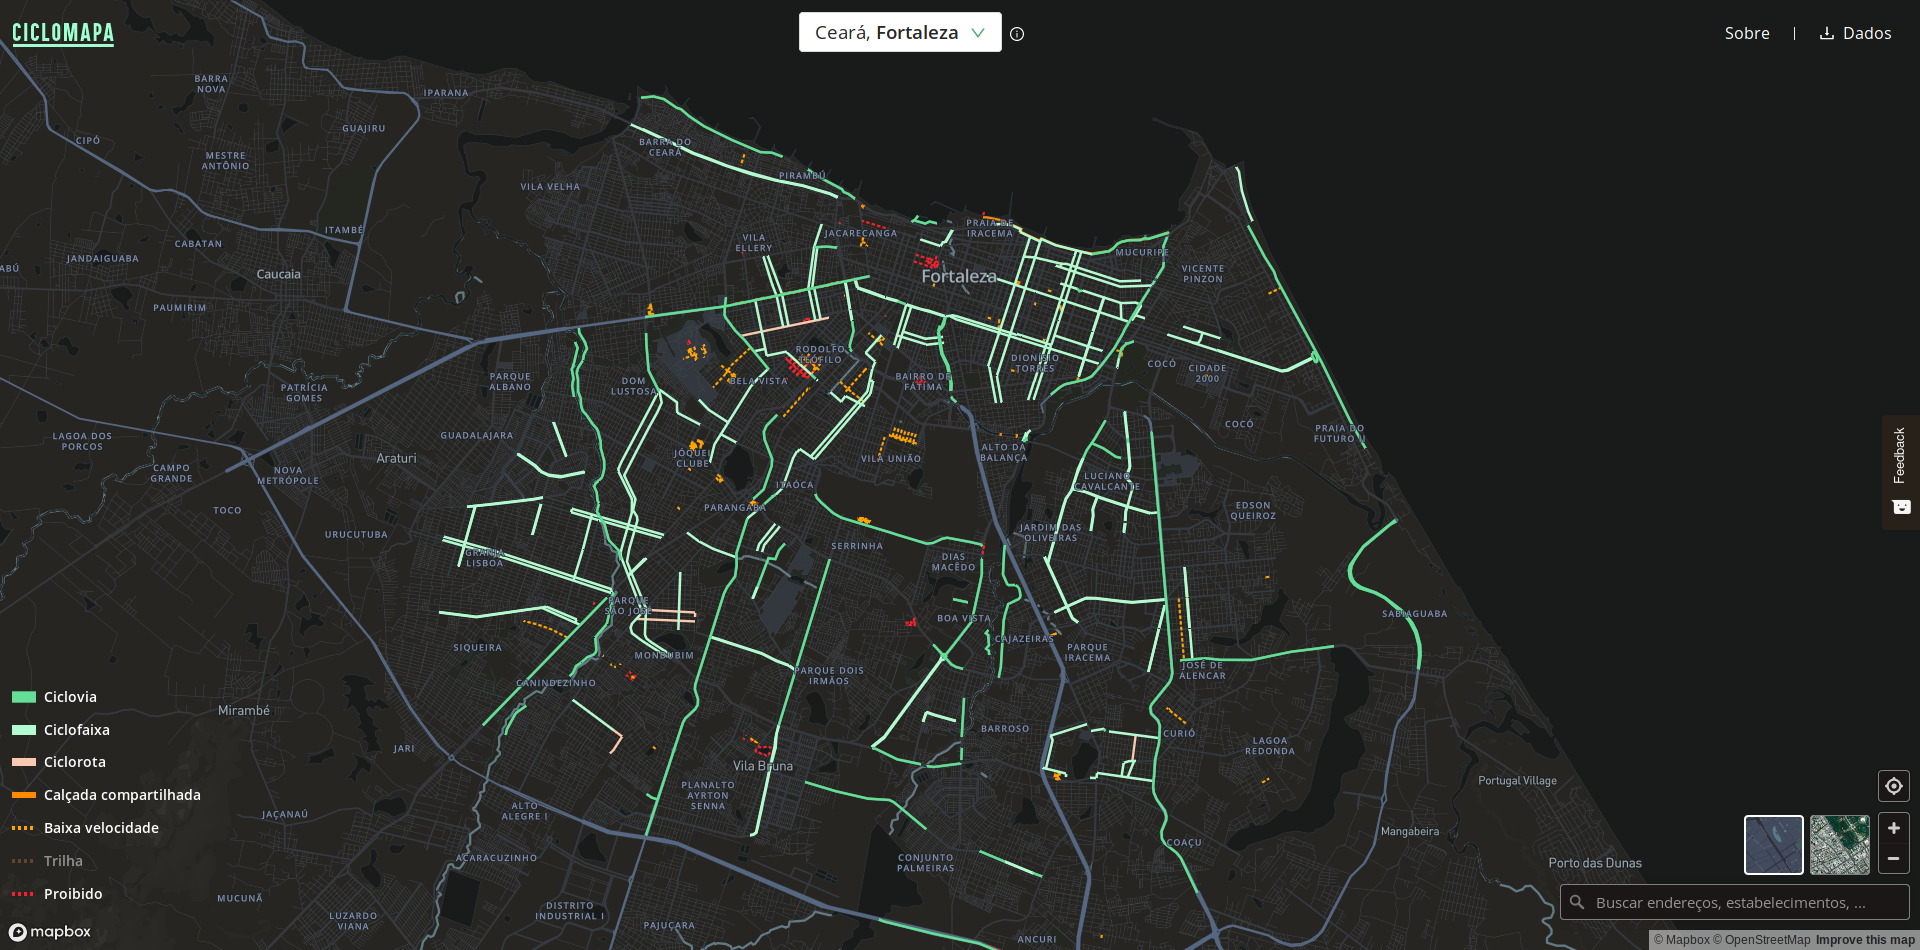
\includegraphics[scale=0.23]{osm_example}
 	\centering
 	\\
 	{Rysunek2. Przykładowy screen z osm}
	\end{figure}
	 
	 Biblioteki: \\
	 
	 
	 
	 
	
	
	
	\newpage
	\renewcommand\refname{Źródła}
	\begin{thebibliography}{}
		\bibitem{vrp} 
		{\hypertarget{optymalizacja}{\textcolor{blue}{
		https://sjp.pwn.pl/slowniki/optymalizacja.html}}}
	
		\bibitem{problemy} 
		{\hypertarget{problemy}{\textcolor{blue}{
		http://www.cs.put.poznan.pl/arybarczyk/TeoriaZlozonosc.pdf}}}
	
		\bibitem{zlozonosc} 
		{\hypertarget{zlozonosc}{\textcolor{blue}{
		http://home.agh.edu.pl/~horzyk/lectures/pi/ahdydpiwykl8.html}}}

		\bibitem{komiwojazer} 
		{\hypertarget{komiwojazer}{\textcolor{blue}{
		Sysło M.M., Deo N., Kowalik J.S., Algorytmy optymalizacji dyskretnej, wyd. drugie, Warszawa: Wydawnictwo Naukowe PWN, 1995, ISBN 83-01-11818-0}}}
	
		\bibitem{dfj}
		{\hypertarget{dfj}{\textcolor{blue}{
		Dantzig, George B. (1963), Linear Programming and Extensions, Princeton, NJ: PrincetonUP, pp. 545–7, ISBN 0-691-08000-3, sixth printing, 1974.}}}
	
		\bibitem{vrp}
		{\hypertarget{vrp}{\textcolor{blue}{
		 Dantzig, George Bernard; Ramser, John Hubert (October 1959). "The Truck Dispatching Problem", https://andresjaquep.files.wordpress.com/2008/10/2627477-clasico-dantzig.pdf}}}
		
		\bibitem{cvrp} 
		{\hypertarget{cvrp}{\textcolor{blue}{T. Ralphs, J. Hartman and M. Galati. "Capacitated Vehicle Routing and Some Related Problems". Some CVRP Slides. Rutgers University. 2001}}}
		
		\bibitem{cvrp2} 
		{\hypertarget{cvrp2}{\textcolor{blue}{https://www.researchgate.net/publication/326129926\_Capacitated\_vehicle\_routing\_problem\\\_model\_for\_carriers}}}
		
		\bibitem{metaheurystyka} 
		{\hypertarget{metaheurystyka}{\textcolor{blue}{Bianchi, Leonora; Marco Dorigo; Luca Maria Gambardella; Walter J. Gutjahr (2009). "A survey on metaheuristics for stochastic combinatorial optimization"}}}
		
		\bibitem{ag} 
		{\hypertarget{ag}{\textcolor{blue}{
		D. E. Goldberg: Algorytmy genetyczne i ich zastosowania. Warszawa: WNT, 1998. (pol.)}}}
	
		\bibitem{python} 
		{\hypertarget{python}{\textcolor{blue}{
		 Guttag, John V. (12.08.2016). Introduction to Computation and Programming Using Python: With Application to Understanding Data. MIT Press. ISBN 978-0-262-52962-4.}}}
	 
	 	\bibitem{osm} 
	 	{\hypertarget{osm}{\textcolor{blue}{
		https://wiki.openstreetmap.org/wiki/About\_OpenStreetMap}}}
		\bibitem{osm} 
		{\hypertarget{osm_example}{\textcolor{blue}{
		https://wiki.openstreetmap.org/wiki/File:Screenshot\_2019-10-23\_CicloMapa.png
		}}}

	\end{thebibliography}
	
	
	%\end{flushleft}
	
\end{document}